\chapter{RESULTS AND DISCUSSIONS}\label{chap5}
\thispagestyle{empty}

The results of the analyses are presented in this chapter divided in to different sections. Each section presents results of one analysis each. 

\section{Sub-figures}

Here we will discuss how to include figures side by side. Assume there are two figures to be added. We have to create \textbf{subfigure} environment inside the figure environment.
\begin{figure}[h]\centering
	\begin{subfigure}[First sub-figure caption] 
	{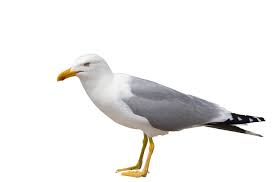
\includegraphics[width=0.40\textwidth]{./picture-files/seagull.jpeg}}
	\end{subfigure}\hfill 
	\begin{subfigure}[Second sub-figure caption] 
	{
\includegraphics[width=0.35\textwidth]{./picture-files/lion.png}}
	\end{subfigure}
	\caption{Common Caption for the Two Figures}
\end{figure}

\section{Tables}
%\pageref{first}

\begin{table}[h] \centering\begin{threeparttable}
\caption[Results of the analysis 1]{Results of analysis to determine the impact of factor A on system performance}
\begin{tabular}{p{2cm}p{2cm}p{2cm}p{2cm}}
\hline Col 1 & Col 2 & Col 3 & Col 4 \\ 
\hline\hline Row 1 & a & b & c \\ 
 Row 2 & A & B & C \\ 
 Row 3 & $\alpha$ & $\beta$ & $\delta$ \\ 
\hline 
\end{tabular} \end{threeparttable}
\end{table}


Another table can be sideways as shown in the next page, Table~\ref{side-tabl}. The table is long and therefore a separate page is used. 


\begin{sidewaystable}[h]
\caption{Performance After Post Filtering} \label{side-tabl}% title name of the table
\centering
% centering table
\begin{tabular}{l c c rrrrrrr}
% creating 10 columns
\hline
\hline
% inserting double-line
Audio &Audibility & Decision &
\multicolumn{7}{c}{Sum of Extracted Bits}
\\[0.5ex]
\hline
% inserts single-line
% Entering 1strow
& & soft & 1 & $-1$ & 1 & 1 & $-1$ & $-1$ & 1\\[-1ex]
\raisebox{1.5ex}{Police} &\raisebox{1.5ex}{5}&hard& 2 & $-4$ & 4 & 4 & $-2$ & $-4$ & 4\\[1ex]
% Entering 2ndrow
& &soft & 1 & $-1$ & 1 & 1 & $-1$ & $-1$ & 1\\[-1ex]\raisebox{1.5ex}{Beethoven} &\raisebox{1.5ex}{5}& hard&8 & $-8$ & 2 & 8 & $-8$ & $-8$ & 6\\[1ex]% Entering 3rd row
& &soft & 1 & $-1$ & 1 & 1 & $-1$ & $-1$ & 1\\[-1ex]\raisebox{1.5ex}{Metallica} &\raisebox{1.5ex}{5}& hard&4 & $-8$ & 8 & 4 & $-8$ & $-8$ & 8\\[1ex]
% [1ex] adds vertical space
\hline % inserts single-line
\end{tabular}
\label{tab:side}
\end{sidewaystable}




\section{Summary}